% GNUPLOT: LaTeX picture with Postscript
\begingroup
  \makeatletter
  \providecommand\color[2][]{%
    \GenericError{(gnuplot) \space\space\space\@spaces}{%
      Package color not loaded in conjunction with
      terminal option `colourtext'%
    }{See the gnuplot documentation for explanation.%
    }{Either use 'blacktext' in gnuplot or load the package
      color.sty in LaTeX.}%
    \renewcommand\color[2][]{}%
  }%
  \providecommand\includegraphics[2][]{%
    \GenericError{(gnuplot) \space\space\space\@spaces}{%
      Package graphicx or graphics not loaded%
    }{See the gnuplot documentation for explanation.%
    }{The gnuplot epslatex terminal needs graphicx.sty or graphics.sty.}%
    \renewcommand\includegraphics[2][]{}%
  }%
  \providecommand\rotatebox[2]{#2}%
  \@ifundefined{ifGPcolor}{%
    \newif\ifGPcolor
    \GPcolortrue
  }{}%
  \@ifundefined{ifGPblacktext}{%
    \newif\ifGPblacktext
    \GPblacktextfalse
  }{}%
  % define a \g@addto@macro without @ in the name:
  \let\gplgaddtomacro\g@addto@macro
  % define empty templates for all commands taking text:
  \gdef\gplbacktext{}%
  \gdef\gplfronttext{}%
  \makeatother
  \ifGPblacktext
    % no textcolor at all
    \def\colorrgb#1{}%
    \def\colorgray#1{}%
  \else
    % gray or color?
    \ifGPcolor
      \def\colorrgb#1{\color[rgb]{#1}}%
      \def\colorgray#1{\color[gray]{#1}}%
      \expandafter\def\csname LTw\endcsname{\color{white}}%
      \expandafter\def\csname LTb\endcsname{\color{black}}%
      \expandafter\def\csname LTa\endcsname{\color{black}}%
      \expandafter\def\csname LT0\endcsname{\color[rgb]{1,0,0}}%
      \expandafter\def\csname LT1\endcsname{\color[rgb]{0,1,0}}%
      \expandafter\def\csname LT2\endcsname{\color[rgb]{0,0,1}}%
      \expandafter\def\csname LT3\endcsname{\color[rgb]{1,0,1}}%
      \expandafter\def\csname LT4\endcsname{\color[rgb]{0,1,1}}%
      \expandafter\def\csname LT5\endcsname{\color[rgb]{1,1,0}}%
      \expandafter\def\csname LT6\endcsname{\color[rgb]{0,0,0}}%
      \expandafter\def\csname LT7\endcsname{\color[rgb]{1,0.3,0}}%
      \expandafter\def\csname LT8\endcsname{\color[rgb]{0.5,0.5,0.5}}%
    \else
      % gray
      \def\colorrgb#1{\color{black}}%
      \def\colorgray#1{\color[gray]{#1}}%
      \expandafter\def\csname LTw\endcsname{\color{white}}%
      \expandafter\def\csname LTb\endcsname{\color{black}}%
      \expandafter\def\csname LTa\endcsname{\color{black}}%
      \expandafter\def\csname LT0\endcsname{\color{black}}%
      \expandafter\def\csname LT1\endcsname{\color{black}}%
      \expandafter\def\csname LT2\endcsname{\color{black}}%
      \expandafter\def\csname LT3\endcsname{\color{black}}%
      \expandafter\def\csname LT4\endcsname{\color{black}}%
      \expandafter\def\csname LT5\endcsname{\color{black}}%
      \expandafter\def\csname LT6\endcsname{\color{black}}%
      \expandafter\def\csname LT7\endcsname{\color{black}}%
      \expandafter\def\csname LT8\endcsname{\color{black}}%
    \fi
  \fi
  \setlength{\unitlength}{0.0500bp}%
  \begin{picture}(7936.00,4250.00)%
    \gplgaddtomacro\gplbacktext{%
      \csname LTb\endcsname%
      \put(816,80){\makebox(0,0)[r]{\strut{}-0.4 $\mu_3$}}%
      \put(816,648){\makebox(0,0)[r]{\strut{}-0.2 $\mu_3$}}%
      \put(816,1216){\makebox(0,0)[r]{\strut{}0 $\mu_3$}}%
      \put(816,1784){\makebox(0,0)[r]{\strut{}0.2 $\mu_3$}}%
      \put(816,2353){\makebox(0,0)[r]{\strut{}0.4 $\mu_3$}}%
      \put(816,2921){\makebox(0,0)[r]{\strut{}0.6 $\mu_3$}}%
      \put(816,3489){\makebox(0,0)[r]{\strut{}0.8 $\mu_3$}}%
      \put(816,4057){\makebox(0,0)[r]{\strut{}1 $\mu_3$}}%
      \put(912,-80){\makebox(0,0){\strut{}0 kg}}%
      \put(1553,-80){\makebox(0,0){\strut{}2 kg}}%
      \put(2195,-80){\makebox(0,0){\strut{}4 kg}}%
      \put(2836,-80){\makebox(0,0){\strut{}6 kg}}%
      \put(3478,-80){\makebox(0,0){\strut{}8 kg}}%
      \put(4119,-80){\makebox(0,0){\strut{}10 kg}}%
      \put(4761,-80){\makebox(0,0){\strut{}12 kg}}%
      \put(5402,-80){\makebox(0,0){\strut{}14 kg}}%
      \put(6043,-80){\makebox(0,0){\strut{}16 kg}}%
      \put(6685,-80){\makebox(0,0){\strut{}18 kg}}%
      \put(7326,-80){\makebox(0,0){\strut{}20 kg}}%
    }%
    \gplgaddtomacro\gplfronttext{%
      \csname LTb\endcsname%
      \put(6912,3914){\makebox(0,0)[r]{\strut{}interpolacja}}%
      \csname LTb\endcsname%
      \put(6912,3754){\makebox(0,0)[r]{\strut{}wynik dodatni}}%
      \csname LTb\endcsname%
      \put(6912,3594){\makebox(0,0)[r]{\strut{}wynik ujemny}}%
      \csname LTb\endcsname%
      \put(1233,3745){\makebox(0,0){\strut{}0.84}}%
      \put(1553,2637){\makebox(0,0){\strut{}0.45}}%
      \put(1874,1472){\makebox(0,0){\strut{}0.04}}%
      \put(3157,1614){\makebox(0,0){\strut{}0.09}}%
      \put(3478,1699){\makebox(0,0){\strut{}0.12}}%
      \put(3798,1472){\makebox(0,0){\strut{}0.04}}%
      \put(5081,1444){\makebox(0,0){\strut{}0.03}}%
      \put(5402,1557){\makebox(0,0){\strut{}0.07}}%
      \put(5723,1472){\makebox(0,0){\strut{}0.04}}%
      \put(7006,1387){\makebox(0,0){\strut{}0.01}}%
      \put(7326,1472){\makebox(0,0){\strut{}0.04}}%
    }%
    \gplbacktext
    \put(0,0){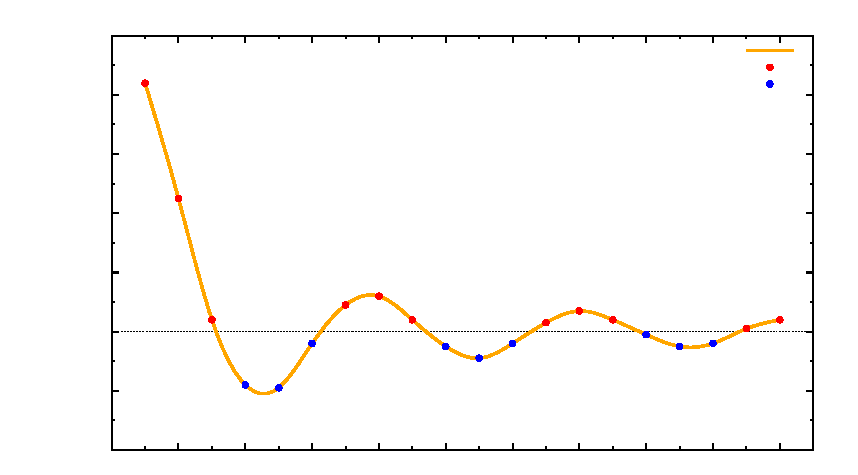
\includegraphics{GNUwykres-gnuplottex-fig7}}%
    \gplfronttext
  \end{picture}%
\endgroup
